% Součást skript na Datové struktury. Viz main.tex
\markright{$ $Id$ $}

\chapter{Trie}

\emph{Trie}\footnote{Název \emph{trie} pochází z anglického 
"re{\bf trie}val", tedy vyzvednutí. Názory na to, jak vyslovovat 
"trie" se různí. V češtině se zpravidla vyslovuje tak jak se píše.} 
je rovinná implementace slovníku.

Máme abecedu $\Sigma$ velikosti $k$. Universum jsou všechna slova nad
$\Sigma$ délky právě $l$ (nekonečnou množinu si nemůžeme dovolit a
kratší slova doplníme zprava mezerami). Chceme reprezentovat množinu
slov $S \subseteq U$.


% --------------------------------------------------------------------------

\section{Základní varianta}

\begin{defn}
\emph{Trie} nad $\Sigma$ je konečný strom, jehož každý vnitřní
vrchol má právě $k$ synů, které jsou jednoznačně ohodnoceny prvky $\Sigma$.
Každému vnitřnímu vrcholu trie odpovídá slovo nad $\Sigma$ délky
nejvýše $l$: kořenu
odpovídá prázdné slovo $\Lambda$; když vrcholu $v$ odpovídá slovo
$\alpha$, pak $v[a]$, synu $v$ ohodnocenému písmenem $a$, odpovídá
slovo $\alpha a$.
\end{defn}

\newcommand{\Nal}{\textrm{Nal}}
\begin{defn}
Řekneme, že trie nad $\Sigma$ \emph{reprezentuje množinu} $S$, když:
\begin{itemize}
  \item Listům je přiřazena boolovská funkce náležení \Nal: $\Nal(t)$ je
  	true právě když slovo, které odpovídá listu $t$, je v $S$.
  \item (\emph{prefixová podmínka}) Když $v$ je vnitřní vrchol trie 
	odpovídající slovu $\alpha$, pak
  	existuje $\beta \in S$ takové, že $\alpha$ je prefix $\beta$.
  \item Pro každé slovo $\alpha \in S$ existuje v trie list odpovídající
  	$\alpha$.
\end{itemize}
\end{defn}

% podle http://en.wikipedia.org/wiki/Trie
\begin{pozn}
Na rozdíl od binárního vyhledávacího stromu (viz kapitola~\ref{bvs},
sekce~\ref{bvs:obecne}), žádný vrchol ve stromě neobsahuje uložený klíč,
který reprezentuje. Namísto toho jeho pozice ve stromě udává klíč, který
reprezentuje\footnote{Tato a následující poznámka jsou volně převzaty z
encyklopedie Wikipedia, heslo Trie.}. 
Pouze některé vrcholy ve stromě obsahují data - např. pro
implementaci slovníku s hesly by data uložená v listech obsahovala popis
tohoho hesla\footnote{Např. slovník spisovatelů, kde listy ve trie by
odpovídaly jménům jednotlivých spisovatelů a data uložená v nich by 
obsahovala seznam jejich děl.}.
\end{pozn}

% podle http://en.wikipedia.org/wiki/Trie
\begin{pozn}
Proč jsou trie výhodné ?

\begin{itemize}
  \item Vyhledávání klíčů je rychlejší než v BVS. Vyhledání klíče délky
  $m$ vyžaduje pouze $O(m)$ času. Pro BVS je to $O(m^2)$ v nejhorším případě,
  protože se musí opakovaně porovnávat počáteční znaky hledaného slova.
  Další výhoda je použití indexace pomocí znaků v operaci MEMBER.
  \item Trie zabírají méně místa. Protože nejsou klíče v trie uloženy
  explicitně, pro uložení jednoho klíče je potřeba pouze amortizovaný
  konstantní prostor.
  \item Pomocí trie lze jednoduše provádět operaci hledání nejdelšího 
  prefixu\footnote{anglicky ``longest-prefix matching``}, kde potřebujeme
  najít klíč, který má nejdelší shodný prefix s hledaným
  klíčem\footnote{To se hodí například pro implementace síťových
  operačních systémů, kde je potřeba provádět tuto operaci pro
  hledání v routovacích tabulkách nebo tabulkách pro překlad adres. 
  V případě směrovacích tabulek se posílá paket na další "hop" podle 
  cílové adresy. Routovací tabulka obsahuje záznamy, které udávají adresu
  sítě a adresu zařízení, na které posílat pakety pro tuto síť - tzv.
  "hop". Tento "hop" se vybírá tak, aby cílová adresa paketu měla
  co možná nejdelší shodný prefix s nějakou adresou sítě v routovací
  tabulce.}. 
  Dále trie dovolují asociovat jednu hodnotu s množinou klíčů, které mají
  shodný prefix\footnote{Tím, že uložíme data do vnitřních uzlů trie.}.
\end{itemize}
\end{pozn}

% ..........................................................................
\subsection{Algoritmus MEMBER}

viz algoritmus \ref{alg:trie.member}.

\begin{algorithm}[!htb]
\caption{MEMBER pro základní verzi trie}
\label{alg:trie.member}
\begin{algorithmic}
\STATE \COMMENT {vyhledání $x = x_1 \dots x_l$}
\STATE $t := \text{kořen}$
\STATE $i := 1$
\WHILE {$t \text{ není list}$}
        \STATE $t := t[x_i]$ // sestup podle znaku $x_i$
        \STATE $i := i + 1$
\ENDWHILE
\STATE \COMMENT {test}
\STATE \textbf{return} $\Nal(t)$
\end{algorithmic}
\end{algorithm}

Na tomto algoritmu je zajímavé to, že používá jednotlivé znaky hledaného
slova $x$ k indexaci v jednotlivých vrcholech trie (viz řádek s
komentářem ve výpisu algoritmu~\ref{alg:trie.member}.). To dovoluje najít
vrchol do kterého se má při hledání sestoupit v čase $O(1)$. Tedy
složitost operace MEMBER je $O(l)$, protože musíme projít nejvýše $l$
vrcholů než dosáhneme listu (délka slov je nejvýše $l$).

% ..........................................................................
\subsection{Algoritmus INSERT}

viz algoritmus \ref{alg:trie.insert}.

\begin{algorithm}[!htb]
\caption{INSERT pro základní verzi trie}
\label{alg:trie.insert}
\begin{algorithmic}
\STATE \COMMENT {vyhledej $x$ pomocí operace MEMBER(x)}
\IF[trie nemusí být tak hluboké, jak potřebujeme] {\textbf{not} $\Nal(t)$}
        \WHILE {$i \leq l$}
                \STATE vrcholu $t$ přidej $k$ listů ohodnocených
                písmeny z $\Sigma$, jejich $\Nal := \textit{false}$
                \STATE $t := t[x_i]$
                \STATE $i := i + 1$
        \ENDWHILE
        \STATE $\Nal(t) := \textit{true}$
\ENDIF
\end{algorithmic}
\end{algorithm}

Při operaci INSERT se sestupuje až na úroveň délky slova, přičemž se
přidávají nové úrovně v případě že nejsou v trie přítomny\footnote{Celkem 
hezky si lze proces přidávání nových hladin v rámci jedné větve představit 
tak, že v každé hladině, která je nově přidaná, "vyroste smeták" s $k$ 
vrcholy.}.

% ..........................................................................
\subsection{Algoritmus DELETE}

viz algoritmus \ref{alg:trie.delete}.

\begin{algorithm}[!htb]
\caption{DELETE pro základní verzi trie}
\label{alg:trie.delete}
\begin{algorithmic}
\STATE \COMMENT {vyhledej $x$ pomocí operace MEMBER(x)}
\IF {$\Nal(t)$}
        \STATE $\Nal(t) := \textit{false}$
        \STATE $t := \text{otec } t$
        \STATE \COMMENT {opravíme prefixovou podmínku}
        \WHILE {všichni synové $t$ jsou listy s $\Nal = \textit{false}$}
                \STATE zruš listy $t$
                \STATE $\Nal(t) := \textit{false}$
                \STATE $t := \text{otec } t$
        \ENDWHILE
\ENDIF  
\end{algorithmic}
\end{algorithm}

Analogicky k operaci INSERT dochází k rušení hladin v rámci jedné větve
v případě že všechny
listy v hladině mají hodnotu $\Nal = \textit{false}$.

Použili jsme obrat $t := \text{otec } t$. To lze provést buď tak, že
se vrchol kromě svých synů odkazuje i na svého otce a spotřebuje tak
paměť navíc, nebo se cesta z kořene do aktuálního vrcholu během
sestupu ve stromu pamatuje na zásobníku. Tento trik se používá u 
všech stromových struktur.

% ..........................................................................
\subsection{Časová a paměťová složitost}

Jedna iterace cyklu zabere konstantní čas. Čas pro MEMBER je $O(l)$,
čas pro INSERT a DELETE je $O(l k)$. Paměťová složitost trie v nejhorším
případě je počet
uložených slov násobený délkou cesty a počtem synů, tedy $O(|S| l k)$.

\begin{pozn}
V případě, kdy S obsahuje (skoro) všechna slova délky $l$, tak může
mít složitost jen $O(|S|)$.
\end{pozn}

% --------------------------------------------------------------------------
\section{Komprimované trie}

Mějme $\Sigma = \{0,1,2\}$, $l=7$.
$S = \{0202011, 0202012, 0202021, 1212102, 1212111, 1212121, 1212122\}$.
Nekomprimované trie pro tuto množinu je na obrázku \ref{fig:tries}.
Vidíme, že písmena na druhé až páté pozici jsou vždy stejná a
% XXX \uv{prokousat} 
předchozí algoritmy se jimi musí prokousat. Přesněji 
řečeno, prohlížení vrcholu $v$, který má jediného 
syna, který není list s hodnotou $\Nal = \textit{false}$, nepřináší 
žádnou kladnou informaci, protože množiny prvků z $S$, 
které jsou reprezentovány vrcholy v podstromu otce $v$ a v podstromu 
vrcholu $v$ jsou stejné. To vedlo k idei tyto vrcholy ze stromu vynechat a
tím zmenšit (komprimovat) trie.  

\begin{figure}
\centering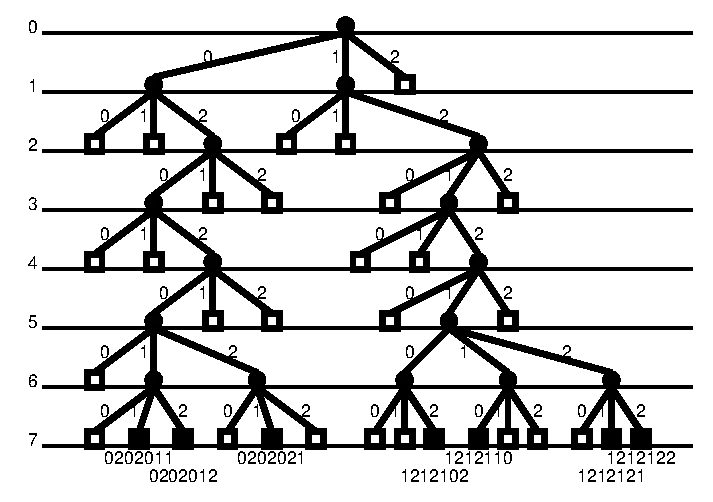
\includegraphics{pics/tries}
\caption{Nekomprimované trie. Černě vyplněné čtverce znázoňují listy,
které odpovíadjí nějakému slovu z (reprezentované) množiny $S$. Tyto listy
mají hodnotu funkce Nal \textit{true}. Bíle vyplněné čtverce žádnému slovu
ze $S$ neodpovídají, mají tedy hodnotu Nal \textit{false}.}
\label{fig:tries}
\end{figure}

\newcommand{\uro}{\textrm{uroven}}
Ke každému vrcholu $v$ přidáme funkci $\uro(v)$ vyjadřující číslo úrovně,
ve které se $v$ nachází v původním trie.
\newcommand{\slo}{\textrm{slovo}}
Ke každému listu $v$ přidáme funkci $\slo(v)$ --- slovo, které odpovídá $v$.

Nyní můžeme vynechávat vrcholy podle následujícího kritéria: 
je-li $v$ vnitřní vrchol a všichni jeho synové kromě $w$ jsou listy s
$\Nal = \textit{false}$, pak $v$ vynech a zařaď $w$ na jeho místo. Tento proces 
opakujeme dokud trie obsahuje nějaký vnitřní vrchol, jehož všichni synové 
s výjimkou jednoho jsou listy, pro něž $\Nal = \textit{false}$. 
Všimněte si, že každý vnitřní vrchol má právě $k$ synů, které jsou 
v jednoznačné korespondenci s písmeny abecedy $\Sigma$.

\begin{priklad}
Nechť $\Sigma = \{0,1,2\}$, $l=3$.
$S = \{ 001,102,010,211,212 \}$.

Nekomprimovaný trie pro množinu $S$ a jeho komprimovaná varianta je na
obr. \ref{fig:tries.compr1}.

\begin{figure}
\centering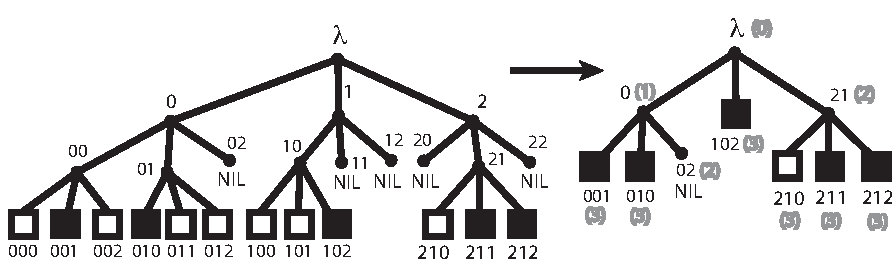
\includegraphics{pics/trie-compr1}
\caption{Komprimace trie. Šedá čísla v závorce značí hodnotu $uroven()$}
\label{fig:tries.compr1}
\end{figure}

\end{priklad}


\begin{pozn}
\mnote{Koubek 2002/2003}
Komprimované trie je tvořený množinou vrcholů, kde pro $\beta$ je
$hladina(\beta) = |\beta|$ a otec $\beta$ je největší vlastní prefix,
který patří do trie + přidané listy. Listy jsou prvky z S + slova $\beta
a$, kde $\beta \in$ trie a $\beta a$ není prefixem žádného slova v $S$. 
Pro prvky z $S$ je Nal = True, jinak false. 
Platí $prvek(\gamma) = \gamma$ pro každý list.

Když $\beta \in$ trie a $a \in \Sigma \rightarrow$
$\Bigl\{$
\begin{tabular}{ll}
$\beta a$ list, & je $a$-tým synem $\beta$ \\
$\exists \delta \in S$, & že $\beta a$ je prefixem $\delta$
\end{tabular}

Potom $a$-tý syn $\beta$ je nejkratší prefix v množině trie v $S$, který
obsahuje $\beta a$.
\end{pozn}

% ..........................................................................
\subsection{MEMBER}

Viz algoritmus \ref{alg:trie.k.mem}

\begin{algorithm}[!htb]
\caption{MEMBER pro komprimované trie}
\label{alg:trie.k.mem}
\begin{algorithmic}
\STATE \COMMENT {vyhledání $x = x_1 \ldots x_l$}
\STATE $t := \text{kořen}$
\WHILE {$t \text{ není list}$}
        \STATE $i := \uro(t) + 1$
        \STATE $t := t[x_i]$ // $x_i$-tý list
\ENDWHILE
\STATE \COMMENT {test}
\STATE \textbf{return} $\Nal(t) \land \slo(t) = x$
\end{algorithmic}
\end{algorithm}

% XXX zde \mnote{něco chybí}

% ..........................................................................
\subsection{INSERT}

Viz algoritmus \ref{alg:trie.k.ins}

\begin{algorithm}
\caption{INSERT pro komprimované trie}
\label{alg:trie.k.ins}
\begin{algorithmic}
\STATE \COMMENT {vyhledej $x$}
\IF {$\Nal(t) \land \slo(t) = x$}
	\STATE \COMMENT {Trie už obsahuje $x$, nedělej nic.}
\ELSE
        \IF {$\slo(t) = x$}
		\STATE \COMMENT {Trie obsahuje správný list,
		pouze nastav příznak. Např. "0202010"}
                \STATE $\Nal(t) := \textit{true}$
	\ELSE
		\STATE \COMMENT {Bude potřeba vložit nový list.}
		\STATE \COMMENT {Najdi, kam ho připojit.}
                \STATE $\alpha$ := nejdelší společný prefix slov
		$x$ a $\slo(t)$. Délku $\alpha$ označme $|\alpha|$.
                \STATE $v$ := vrchol na cestě z kořene do $t$ takový,
                že $\uro(v)$ je největší, která je $\leq |\alpha|$
                \IF {$\uro(v) = |\alpha|$}
                        \STATE \COMMENT {$v$ je otec nového listu}
		\ELSE[$\uro(v) < |\alpha|$]
                        \STATE \COMMENT {Bude potřeba vytvořit
			otce nového listu}
                        \STATE $a$ := $\uro(v)+1$-ní písmeno $\alpha$
                        \STATE $u := v[a]$
                        \STATE \COMMENT {Mezi $v$ a $u$ vytvoř nový
			vnitřní vrchol odpovídající slovu $\alpha$}
                        \STATE $w$ := nový vrchol, $\uro(w) := |\alpha|$
                        \STATE $v[a] := w$
                        \STATE $c$ := $|\alpha|+1$-ní písmeno $\slo(t)$
                        \STATE $w[c] := u$
                        \FORALL {$b \in \Sigma, b \neq c$}
                             \STATE $z$ := nový vrchol, $\uro(z) := |\alpha|+1, \Nal(z) := \textit{false}, \slo(z) := \alpha b$, 
                             \STATE $w[b] := z$
                        \ENDFOR
                        \STATE $v := w$
                \ENDIF
		\STATE \COMMENT {Správnému listu přiřaď $x$}
		\STATE $d$ := $|\alpha|+1$-ní písmeno $x$
                \STATE $s := v[d]$
                \STATE $\uro(s) := l, \Nal(s) := \textit{true}, \slo(s) := x$
        \ENDIF
\ENDIF
\end{algorithmic}
\end{algorithm}

% ..........................................................................
\subsection{DELETE}

Viz algoritmus \ref{alg:trie.k.del}

\begin{algorithm}[!htb]
\caption{DELETE pro komprimované trie}
\label{alg:trie.k.del}
\begin{algorithmic}
\STATE \COMMENT {vyhledej $x$}
\IF {$\Nal(t) \land \slo(t) = x$}
        \STATE $u$ := otec $t$
        \STATE $i := \uro(u)$
        \STATE $\Nal(t) := \textit{false}$
        \STATE $\uro(t) := i+1$, $\slo(t)$ := prefix slova $x$ délky $i+1$
        \STATE \COMMENT {vrchol $u$ má alespoň jednoho syna, který není list s $\Nal = \textit{false}$}
        \IF {všichni synové $u$ kromě syna $w$ jsou listy s $\Nal = \textit{false}$}
                \STATE $v$ := otec $u$
                \STATE smaž $u$ a všechny syny $u$ kromě $w$
                \STATE $j := \uro(v) + 1$
                \STATE $v[x_j] := w$ // $x_j$-tý syn $v$ je $w$
        \ENDIF
\ENDIF  
\end{algorithmic}
\end{algorithm}

% ..........................................................................
\subsection{Časová a paměťová složitost}

Paměťová složitost takto komprimovaných trie je $O(nk)$, kde 
% oprava by Ladislav Prosek O(nl + kl) -> O(nk)
$n$ je velikost reprezentované množiny. (maximálně $n-1$ vnitřních vrcholů,
každý s polem délky $k$).
Časová složitost operace MEMBER je v nejhorším
případě $O(l)$, pro INSERT a DELETE je to $O(l+k)$. 
(může být nutné přidat/odebrat jeden vnitřní vrchol).
% oprava slozitosti v nejhorsim pripade by Ladislav Prosek 

V průměrném případě (za předpokladu rovnoměrného
rozložení vstupních dat) je to očekávaná hloubka trie. Tu
teď spočítáme.

Nechť
\[
q_d = \pr(\text{trie má hloubku alespoň $d$})
\]
Očekávaná hloubka trie reprezentující $n$ slov je
\[
E_n = \sum_{d=0}^\infty d (q_d - q_{d+1}) = \sum_{d=0}^\infty q_d
\]
Když funkce $\text{pref}_{d-1}$, přiřazující slovu 
$\alpha$ jeho prefix délky $d-1$, je na množině $S$ prostá,
pak trie reprezentující množinu $S$ má hloubku nejvýše $d$.
Spočítáme počet množin o velikosti $n$, na nichž je funkce $\text{pref}_{d-1}$ 
prostá. Tyto množiny získáme tak, že vybereme $n$ prefixů délky $d-1$
a každý doplníme všemi sufixy délky $l-d+1$. Proto těchto množin je
\[
\binom{k^{d-1}}{n} k^{n (l-d+1)}.
\]
Protože všech podmnožin velikosti $n$ je $\binom{k^l}{n}$ dostáváme, že 
\begin{align*}  
q_d 
 &\leq 1 - \frac{\binom{k^{d-1}}{n} k^{n (l-d+1)}}{\binom{k^l}{n}} 
\Biggl\} \text{pravděpodobnost} \\
 &\leq 1 - \frac{k^{d-1}(k^{d-1}-1)\dots(k^{d-1}-(n-1)) k^{n(l-d+1)}}{k^{ln}}\\
 &   = 1 - \prod_{i=0}^{n-1} \left( 1 - \frac{i}{k^{d-1}} \right) \\
 &\leq 1 - \exp\left( \frac{-n^2}{k^{d-1}} \right)\\
 &\leq \frac{n^2}{k^{d-1}},
\end{align*}
poněvadž
\begin{align*}
                  \prod_{i=0}^{n-1}    \left( 1 - \frac{i}{k^{d-1}} \right)
 &   = \exp\left( \sum_{i=0}^{n-1} \ln \left( 1 - \frac{i}{k^{d-1}} \right)
	   \right)\\
 &\geq \exp\left(         \int_0^n \ln \left( 1 - \frac{i}{k^{d-1}} \right)
	   \right)\\
 &   = \exp\left( \frac{-n^2}{k^{d-1}} \right),
\end{align*} 
(užijte integrální kriterium a substituci $x = k^{d-1}(1-t)$) a 
$e^x - 1 \geq x$ (odtud $1 - e^x \leq -x$). 
Tedy pro $c = 2\lceil \log_kn\rceil$ dostáváme

\begin{align*}
E_n
 & = \sum_{d=1}^cq_d + \sum_{d=c+1}^{\infty}q_d\\
 &\leq c + \sum_{d=c}^{\infty}\frac{n^2}{k^d}\\
 &\leq 2\lceil\log_kn\rceil +
		\left( \frac{n^2}{k^c} \right) \sum_{d=0}^{\infty} k^{-d}\\
 &\leq 2\lceil\log_kn\rceil + \frac{1}{1-1/k}\\
 & = 2\lceil\log_kn\rceil + \frac{k}{k-1}.
\end{align*}

Tedy očekávaný čas operace MEMBER je $O(\log_k(n))$ ($O(\frac{\log n}{\log
k})$)
a $O(\log_k(n) + k)$ pro INSERT a DELETE
\mnote{L.Prošek: Možná v té očekávané složitosti by šlo +k zanedbat, ale
ne na základě toho tvrzení, které dokazuje jen očekávanou hloubku}
pro komprimované trie (za předpokladů rovnoměrného rozložení vstupních dat) 
Zde parametr $k$ vyjadřuje vztah mezi prostorovými 
a časovými nároky.

% . . . .. . . .. .. .. . .  . .. .. .. . . ..  ..  .... . . .. . .. . .
% nasledujici sekci (jeste kompr. trie atd.) dopsal Vladimir Kotal, 2003

\begin{algorithm}[!htb]
	\caption{INSERT pro komprimované trie, analogie \ref{alg:trie.k.ins} (verze Koubek 2002)}
\label{alg:trie.k.ins_unk}
\begin{algorithmic}
\STATE INSERT($x=x_1, ..., x_l$)
\STATE $t$ $\leftarrow$ kořen
\WHILE {$t$ neni list}
  \STATE i $\leftarrow$ hladina($t$), $t$ $\leftarrow$ $(a_{i+1})$-ní syn $t$
\ENDWHILE
\IF {prvek($t$) neni prefix $x$}
  \STATE $\beta$ = největší společný prefix $x$ a prvek(t)
  \STATE $\beta a$ = prefix $\alpha$
  \STATE $\beta b$ = prefix prvek($t$)
  \STATE while $hladina(t) > |beta|$ do t $\leftarrow$ otec(t) done
  \IF {$hladina(t) < |\beta|$}
    \STATE vytvoříme nový vrchol $w$, jehož synové, kromě $b$-tého syna budou listy s
    \STATE funkcemi Nal = false
    \STATE $prvek(t) = \beta$ + oznaceni syna
    \STATE $hladina(w) = |\beta|, \beta = (a_1, ..., a_i)$
    \STATE necht $v = a_{hladina(t) + 1}$ - tý syn t, b-tý syn w je v
    \STATE $w = a_{hladina(t)+1}$-tý syn t
  \ENDIF
  \STATE z $\leftarrow$ a-tý syn $t$, Nal($z$) = true, prvek($z$) = $x$
\ELSE
  \STATE Nal(t) = true, prvek(t) = $x$
\ENDIF
\end{algorithmic}
\end{algorithm}


\mnote{XXX dalsi neznamy algoritmus z prednasky 2002}
\begin{algorithm}[!htb]
\caption{DELETE pro komprimované trie (?)}
\label{alg:trie.k.del_unk}
DELETE($x=x_1, ..., x_l$)
\begin{algorithmic}
\STATE t $\leftarrow$ kořen
\WHILE {t neni list}
  \STATE i $\leftarrow$ hladina(t), t $\leftarrow$ $(a_{i+1}$-ni syn t
\ENDWHILE
\IF {Nal(t) = true a prvek(t) = j} 
  \STATE Nal(t) = false
  \STATE v $\leftarrow$ otec(t)
  \STATE prvek(t) $\leftarrow$ prefix prvek(t) o délce hladina v+1
  \IF {vsichni synove vrchovlu v az na jednoho jsou listy s Nal = false}
    \STATE w $\leftarrow$ syn(v), ktery je bud list s Nal(w) = true nebo neni list
    \STATE necht v je a-tý ($a_i$-ty ???) syn svého otce, v smažeme a smažeme
    \STATE všechny syny $v \neq w$
    \STATE w $\leftarrow$ a-tý ($a_i$-tý ???) syn otce v
  \ENDIF
\ENDIF
\end{algorithmic}
\end{algorithm}


\section{Ještě komprimovanější trie}

% XXX dopsat !
\begin{priklad}
\label{example.trie.yetmorecompr}

\begin{figure}[!htb]
\centering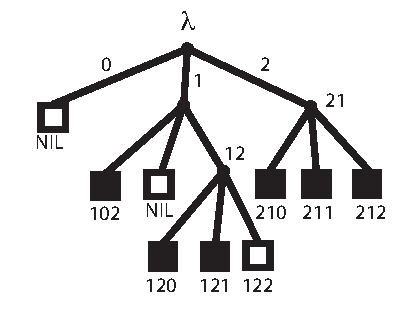
\includegraphics{pics/trie-compr2}
\caption{Nekomprimovaný trie pro příklad \ref{example.trie.yetmorecompr}}
\label{fig.trie.compr}
\end{figure}

Mějme komprimovaný trie z obr. \ref{fig.trie.compr}
a jeho matici: 

\hspace{5mm}

\begin{tabular}{|l|l|l|l|}
\hline
 & 0 & 1 & 2 \\
\hline
root & NIL & a & b \\
a & 102 & NIL & c \\
b & 210 & 211 & 212 \\
c & 120 & 121 & NIL \\
\hline
\end{tabular}
\end{priklad}

\hspace{5mm}

Chceme se zbavit položek NIL v matici reprezentující trie. Další komprese
dosáhneme pomocí vektorů $hod$ (vektor hodnot) a $rd$. Tyto vektory budou
reprezentovat původní matici.

\mnote{co znamena $rd$ ?}

\subsection{Popis $A$ a $rd$}

Zpět k našemu příkladu:

\begin{enumerate}
\item
  \begin{tabular}{|l|llllll|}
  \hline
  hod & 210 & 211 & 212 & 120 & 121 & NIL \\
  \hline
  \end{tabular}
  
  \hspace{2mm}
  
  \begin{tabular}{|l|llll|}
  \hline
     & root & a & b & c \\
  \hline
  rd &      &   & 0 & 3 \\
  \hline
  \end{tabular}
  
  % \hspace{5mm}
  
\item  
  \begin{tabular}{|l|llllllllll|}
  \hline
  hod & 210 & 211 & 212 & 120 & 121 & a & b & 102 & NIL & c \\
  \hline
  \end{tabular}
  
  \hspace{2mm}
  
  \begin{tabular}{|l|llll|}
  \hline
     & root & a & b & c \\
  \hline
  rd & 4    & 7 & 0 & 3 \\
  \hline
  \end{tabular}
\end{enumerate} 
%  \hspace{5mm}

Řádek $i$ začíná na místě $rd(i)$ a musí být splněna podmínka: \\
Když $M_{i,j} \neq NIL \neq M_{i',j'}$, pak $rd(i) + j \neq rd(i') + j'$ \\
Když na místě hod chceme zapsat prvek $\neq NIL$ a NIL, pak zapíšeme prvek
$\neq NIL$.

% ------------------------------------------------------------------------

\subsection{Algoritmus pro hledání rd a hod}

% XXX r x s
Nechť $M$ je matice typu $r x s$, má $m$ významných míst $\neq$ NIL.

\begin{itemize}
\item pro každý řádek nalezneme počet míst $\neq$ NIL
\item setřídíme řádky Bucketsortem, tak že rádky s~větším počtem míst
 $\neq$ NIL předcházejí řádky s menším počtem míst $\neq$ NIL
\item procházíme řádky v daném setřídění a pro každý řádek $i$ nalezneme
  nejmenší číslo $rd(i)$, že nedochází ke kolizi s předchozími řádky (tj.
  když $M_{i',j'} \neq NIL \neq M_{i,j}$) a řádek $i'$ byl zařazen, pak
  $rd(i) + j \neq rd(i') + j'$.
  Pak $M_{i,j} \neq NIL$ je uloženo ve vektoru hod na místě $rd(i)+j$.
\end{itemize}

$m(l)$ - počet míst $\neq$ NIL v řádcích s počtem míst $\geq l+1 \neq NIL$.

\begin{theorem}
Když $m(l)(l+1) \leq m$ pro každé $l$, pak $rd(i) < m$ pro každý řádek $i$
a algoritmus vyžaduje čas $O(rsm)$.
\end{theorem}

\begin{proof}
Předpokládejme, že hledáme rd pro řádek $i$, který má l míst $\neq NIL$. \\
ve vektoru hod je obsazeno méně než $m(l-1)$ míst. \\ 
zkoušíme $rd(i)=1,2,...$ \\
$rd(i) = 1,2,...$ je zakázané, když vznikne kolize. \\
tj. $\exists$ řádek $i'$ předcházející a $\exists j,j'$ takové, že
$M_{i',j'} \neq NIL \neq M_{i,j}$ 
a platilo by $rd(i') + j' = rd(i) + j$.
$\rightarrow$ těchto možností je $< lm(l-1) \leq m$. \\
$O(rs)$ - zjistíme pro každý řádek počet míst $\neq NIL$. \\
$O(m+r)$ - třídění Bucketsortem \\
$O(mrs)$ - krok 2
\end{proof}

%jedna možnost
%% XXX obr. matice
%M = 
%$\rightarrow$ budeme mít moc řádků - nevhodné

\begin{priklad}
XXX nejaky komentar \\

\vspace{5mm}

\begin{tabular}{|l|lll|}
\hline
M & 0 & 1 & 2 \\
\hline
root & NIL & a & b \\
a & 102 & NIL & c \\
b & 210 & 211 & 212 \\
c & 120 & 121 & NIL \\
\hline
\end{tabular}

\vspace{5mm}

\begin{tabular}{|l|llll|}
\hline
    & root & a & b & c \\
\hline
rd  &    4 & 7 & 0 & 3 \\
\hline
\end{tabular}

\vspace{3mm}

\begin{tabular}{|l|llllllllll|}
\hline
hod & 210 & 211 & 212 & 120 & 121 & a & b & 102 & NIL & c \\
\hline
\end{tabular}

\vspace{3mm}

\begin{tabular}{|l|lll|}
\hline
M' & 0 & 1 & 2 \\
\hline
b & 210 & 211 & 212 \\
c & 120 & 121 & NIL \\
root & NIL & a & b \\
a & 102 & NIL & c \\
\hline
\end{tabular}

\hspace{3mm}

(přehodili jsme pouze řádky)

$sl$ - vektor posunutých sloupců

\begin{itemize}
\item $sl(0) = 0$
\item $sl(1) = 1$
\end{itemize}

\begin{tabular}{|l|lll|}
\hline
M' & 0 & 1 & 2 \\
\hline
1 & 210 & NIL & NIL \\
2 & 120 & 211 & 212 \\
3 & NIL & 121 & NIL \\
4 & 102 & a & b \\
5 & NIL & NIL & c \\
\hline
\end{tabular}

\hspace{5mm}

\begin{tabular}{l}
$zac = (6,0,6,3,6)$ \\
$hod = (120, 211, 212, 102, a, b, 210, 121, c)$
\end{tabular}

Když $M(i,j)$ je významné místo, pak $M(i,j) = hod(zac(i+sl(j)) + j)$.

\subsection{Vertikální posun sloupců}

$cd$ - vektor sloupcového posunutí, slouží k zápisu transformace

\vspace{5mm}

\begin{tabular}{|l|lll|}
\hline
   & 0 & 1 & 2 \\
\hline
cd & 0 & 1 & 2 \\
\hline
\end{tabular}
\par

\vspace{5mm}

\begin{tabular}{|l|lllll|}
\hline
   & 0 & 1 & 2 & 3 & 4 \\
\hline
rd & 6 & 0 & 6 & 3 & 6 \\
\hline
\end{tabular}
\par

\vspace{5mm}

\begin{tabular}{|l|lllllllll|}
\hline
hod & 120 & 211 & 212 & 102 & a & b & 210 & 121 & c \\
\hline
\end{tabular}

\hspace{3mm}

\end{priklad}

Jak najdeme nazpátek místa ? Platí, když $M_{i,j} \neq NIL$, pak
$hod(rd(i+cd(j)+j)) = M_{i,j}$
\mnote{je ten vzorec správně ?}

\par
{\em značení:} 
\begin{itemize}
\item f(-,-) je fce dvou proměnných 
\item $B_j$ matice posunutých prvních sloupců 
\item $m_j$ počet míst $\neq NIL$ v $B_j$ 
\item $m_j(l)$ počet míst $\neq NIL$ v řádcích matice $B_j$, které mají aspoň l+1 míst $\neq NIL$
\end{itemize}
\par

Budeme chtít, aby $\forall j \forall l$ platilo $m_j(l) \leq
\frac{m}{f(l,m_j)}$. \\
Okrajové podmínky na f: f musí splňovat:
\begin{itemize}
\item $\forall$ l platí $f(l,m) \geq l+1$
\item$\forall$ j platí $f(0,m_j) \leq \frac{m}{m_j}$
\end{itemize}

\subsubsection{Algoritmus na posunutí sloupců}

\begin{enumerate}
\item Pro každý sloupec v pořadí $0,1,...$ nalezneme nejmenší $cd(j)$ 
takové, aby matice $B_j$ splňovala 
$\forall l$ $m_j(l) \leq \frac{m}{f(l,m_j)}$
(každý sloupec posunujeme dokud nesplňuje podmínku) 
\item Na získanou matici $B = B_s$ pak použijeme předchozí algoritmus. 
\end{enumerate}

Platí $m(l) = m_s(l) \leq \frac{m}{f(l,m)} \leq \frac{m}{l+1}$. \\
Hledáme hodnotu $cd(j)$ a předpokládáme, že pro nějakou hodnotu 
$cd(j)$ není splněna
podmínka pro $l$, tj. platí $m_j(l) > \frac{m}{f(l,m)}$
... platila pro $B_{j-1}, tj. m_{j-1}(l) \leq \frac{m}{f(l,m_{j-1})}$
\par
Z toho plyne $m_j(l) - m_{j-1}(l) > \frac{m}{f(l,m_j)} -
\frac{m}{f(l,m_{j-1}}$.
\par

Jak roste číslo $m_j(l)$ ? 
\begin{enumerate}
\item v matici $B_{j-1}$ existuje řádek s aspoň $l+1$ místy $\neq NIL$ 
a s tímto řádkem se střetne místo $\neq NIL$ (v $j$-tém sloupci 
$\leftarrow m_{j-1}(l)$
vzroste o $1$)
\item v matici $B_{j-1}$ existuje řádek s $l$ místy $\neq NIL$ a s tímto
řádkem se střetne místo $\neq NIL$ v $j$-tém sloupci. Pak $m_{j-1}(l)$
vzroste o $l+1$.
\end{enumerate}

střet - řádek v $B_{j-1}$ s aspoň $l$ místy $\neq NIL$ a místo $\neq NIL$
v $j$-tém sloupci. Aby nebyla splněna podmínka pro l, musí být počet střetů
pro danou hodnotu $cd(j)$
být aspoň 
$$\frac{\frac{m}{f(l,m_j)} - \frac{m}{f(l,m_{j-1})}}{l+1}$$
\par
V matici $B_{j-1}$ je nejvýše $\frac{m_{j-1}(l-1)}{l} \leq \frac{m}{l
f(l-1,m_{j-1}}$ řádků s aspoň $l$ místy $\neq NIL$, v j-tém sloupci je $m_j -
m_{j-1}$ míst $\neq NIL$. \\
\par

Podmínka pro $l$ může zakázat nejvýše 
\begin{multline}\bigparens
\frac{ \frac{m(m_j - m_{j-1})}{l f(l-1,m_{j-1}} }
  { \frac{ \frac{m}{f(l,m_j} - \frac{m}{f(l,m_{j-1}} }{l+1} } 
\text{ hodnot cd} = 
\frac{l+1}{l} \frac{((m_j - m_{j-1})}{\frac{f(l.m_{j-1})}{f(l,m_j)} - 1}
  \frac{f(l.m_{j-1})}{f(l,m_{j-1})}
\end{multline}
\par

Stačí nám sčítat přes hodnoty $l$ takové, že \\
$m m_{j-1}(l) \leq l+1$ tj. přes 
$l \leq l_0 = min\{l; \frac{m}{f(l,m_{j-1}} < l\}$, \\
$m_{j-1}(l) \leq \frac{m}{f(l,m_{j-1})} \leq l+1$.

Celkový počet zakázaných hodnot $cd$ je menší než 
\begin{multline}
\label{odh-zak-hodnot}\bigparens
\sum_{l=0}^{l_0} \frac{l+1}{l} \frac{(m_j - m_{j-1})}{
\frac{f(l,m_{j-1}}{f(l,m_j)} - 1} \frac{f(l,m_{j-1}}{f(l-1,m_{j-1}}
\end{multline}

Zvolíme $f(l,m_j) = 2^{l(2 - \frac{m_j}{m})}$.

\begin{pozn}
Jelikož se $f$ vyskytuje v sumě jen v podílech, výraz se zjednodušší,
zvolíme-li $f(l, m_j) = 2^{g(l, m_j)}$, kde g je nějaká vhodná funkce.
Dosadíme-li, můžeme si všimnout, že dostaneme v exponentech rozdíly 
$g(l, m_{j-1}) - g(l, m_j) a g(l, m_{j-1}) - g(l - 1, m_{j-1})$,
které vznikly vhodnou předchozí úpravou výrazu.

(... suma z Mehlhorna na straně 10, třetí suma od spoda ...)
\par

Teď se lze zbavit $-1$ ve jmenovateli použitím nerovnosti 
$2^x - 1 = e^{x\ln2} - 1 \geq x\ln2$.

(... suma z Mehlhorna na straně 10, druhá suma od spoda ...)
\par
Dalším pozorovaním zjistíme, že v takto získaných rozdílech se mění
jenom jedna proměnná. \\
Výraz se dále zjednodušší, bude-li $g(l, m_j) = h(l)k(m_j), kde h(l), k(m_j)$
budou vhodné lineární funkce. \\
U funkce k linearitou využijeme rozdílu $m_{j-1} - m_j$ v čitateli, který
teď můžeme zkrátit.

(... suma z Mehlhorna na straně 10, první suma od spoda ...)
\par
Dalšími heuristikami a s využitím okrajových podmínek pro $f$ nakonec
zjistíme, že dobrou volbou jsou funkce $h(l) = l, k(m_j) = 2 - \frac {m_j}m.$
\end{pozn}
 
Takto definovaná f splňuje okrajové podmínky: \\
$f(l,m) = 2^l \geq l+1$ $\forall l=0,1,...$ \\
$f(0,m_j) = 1 \leq \frac{m}{m_j}$ $\forall j=0,1,...,s$

dosadíme do odhadu \ref{odh-zak-hodnot} a dostaneme 

\begin{multline}
\sum_{l=1}^{l_0} 
  \frac{l+1}{l} 
  \frac
    {(m_j - m_{j-1})}
    { 2^{l ( \frac{m_j}{m} - \frac{m_{j-1}}{m} ) }}
  2^{( 2 - \frac{m_{j-1}}{m} )} \leq \\
\text{využijeme, že $2^x - 1 \geq x ln(2)$} \\
\sum_{l=1}^{l_0} 
  \frac{l+1}{l} 
  \frac{(m_j - m_{j-1})}{l( \frac{m_j}{m} - \frac{m_{j-1}}{m} )} 4 = \\
\frac{4m}{ln(2)} \sum_{l=1}^{l_0} 
  \frac{l+1}{l^2} = \frac{4m}{ln(2)} (\sum_{l=1}^{l_0} \frac{1}{l} +
  \sum_{l=1}^{l_0} \frac{1}{l^2}) \leq \\
\text{integrální kriterium} \\
\frac{4m}{ln(2)} (1 + ln(l_0)) + \frac{\pi^2}{6} \leq 4m \log_2(l_0) +
15.3m \\
\text{odhadneme $l_0$: } 
l_0 = min\{l; \frac{m}{f(l,m_{j-1}} < l\} \rightarrow l_0 < \log(m) \\
\text{pak } \leq 4m\log \log m) + 15.3m
\end{multline}

Celý algoritmus spočítá uložení matice $M$ typu $r \times s$ do vektorů  \\
$cd$ - dimenze $s$, \\
$rd$ - dimenze $4m\log \log m) + 15.3m + r$, \\
$hod$ dimenze $m+s$, \\
přitom hodnoty $cd(j) < 4m\log \log m) + 15.3m$ a $rd(i) < m$.
\par
Čas potřebný k výpočtu je $O(sr(m \log \log(m))^2)$, kde $m$ je počet míst $\neq
NIL$ v matici $M$.


\subsection{Úsporné uložení řídkého vektoru}

Máme vektor v dimenze $n \cdot d$ (rozdělený na $n$ bloků velikosti $d$)
a $i_0 < i_1 < ... < i_{t-1}$ jsou všechny
indexy $i$ takové, že $v(i) \neq 0$. \\
Vytvoříme vektor $cv$ dimenze $t$, $cv(j)=v(i_j)$. \\
Náš úkol - pro dané l zjistit, zda $l = i_j$ a případně nalézt toto $j$. \\
Sestavíme vektor $base$ dimenze $n$:

\vspace{1mm}

${\rm base(j) = }$
% \left 
$\Bigl\{$
\begin{tabular}{ll}
-1 & $i_k$ {\tt div} $d \neq j$, $\forall k=0,1,...,t-1$ \\
$min\{l; i_l {\tt div} d = j\}$ & $\exists l$, že $i_l$ {\tt div} $d = j$ \\
\end{tabular}
% \right. 

\vspace{1mm}

a matici $offset$ typu $n \times d$ 

\vspace{1mm}

${\rm offset(j,k) =}$
% \left 
$\Bigl\{$
\begin{tabular}{ll}
-1 & $i_l \neq jd+k$, $\forall l = 0,1,...,t-1$ \\
$l-base(j)$ & $i_l = jd+k$ \\
\end{tabular}

\vspace{2mm}

Nyní uložíme matici $offset$ do vektoru $off$ dimenze $n$
tak, že z každého řádku vytvoříme číslo $v$ soustavě o základu $d+1$: \\

off(j) = $\sum_{k=0}^{d-1}(offset(j,k) + 1)(d+1)^k$ \\
potřebujeme $base(dim n)$, $off(dim n)$ \\
smysluplné když $d \ll n$ a $t < n$ (např. $d = \log \log n)$)

Platí následující vztahy: 
\begin{enumerate}
\item $v(h) = 0 \leftrightarrow offset(h {\tt div} d, h \bmod d) = -1$
\item $v(h) = 1 \rightarrow h = base(h {\tt div} d) + offset(h {\tt div} d, h
\bmod d)$
\item $offset(i, j) = off(i) {\tt div} (d+1)^j \bmod (d+1) - 1$
\end{enumerate}
\par

pro dané $i$ - nalezení hodnoty $v(i)$
když $base(i {\tt div } d) = -1$, pak $v(i) = 0$ \\
$base(i {\tt div } d) \neq -1$, pak $k = i \bmod d$ \\
$j = i {\tt div } d$ \\
$l = off(j) {\tt div } (d+1)^k$ \\
$l = l \bmod (d+1)$ \\
$l = l - 1 + base(j)$ \\
$v(i) = cv(l)$ \\

Lze použít pro malé $t$ a $(d+1)^d$ v rozsahu velikosti registru - vhodné
např. pro $d \approx \log \log n)$.

\begin{priklad}
XXX uvod k prikladu

$v$ = 
\begin{tabular}{|l|l|l|l|}
\hline
0 1 0 & 1 0 1 & 0 0 0 & 0 0 1 \\
\hline
      0  &     1 &      -1 &    3 \\
\hline
\end{tabular}

\vspace{5mm}

$i_0 = 1$, $i_1 = 3$, $i_2 = 5$, $i_3 = 11$, $d = 3$ \\

$cv$ = 
\begin{tabular}{|l|l|l|l|}
\hline
v(1) & v(3) & v(5) & v(11) \\
\hline
\end{tabular}

\vspace{5mm}

$base$ =
\begin{tabular}{|l|l|l|l|}
\hline
0 & 1 & -1 & 3 \\
\hline
\end{tabular}

\vspace{5mm}

\begin{tabular}{|l|llll|}
\hline
offset & 0 & 1 & 2 & 3 \\
\hline
0 & -1 & 0 & -1 & -1 \\
1 & 0 & -1 & -1 & -1 \\
2 & -1 & 1 & -1 & 0 \\
\hline
\end{tabular}

\vspace{5mm}

3. sloupec tabulky offset repr. nuly \\
\noindent
off = 
\begin{tabular}{|l|l|l|l|}
\hline
4 & 33 & 0 & 16 \\
\hline
\end{tabular}

\vspace{5mm}

Potom
$off(7) = (offset(1,0) + 1)4^0 + (offset(1,1) + 1)4^1 + (offset(1,2) +
1)4^2$
$off(1) = 1 + 0 + 2\cdot4^2 = 33$

\end{priklad}
